\section{Material} \label{material}
The experiements is conducted in Lam Thao District, Phu Tho province, Vietnam. This part is favorable for its location within the Red River delta, under the influence of tropical weather and sustain 1720 mm of annual rainfall. It have been ultilised by local residents for cultivating rice for years. Our sample rice field is sepperated into 54 part of 100m2 square parcels. With the help of locals farmer, the parcels are fertilized into differents amounts of N, P, K which will cause variation in leaf's spectral reflectance. The farmers was also request for their expertises to take care of the rice field during its growth stages to minimize the crops harms because of water stress or diseases. In each divided parcels, the data is extracted 3 times using specialised machine for measuring spectral reflectance.

The data is captured into a folder with two types of files: a set of sed files and csv file. The sed files are taken from the specialised machine while contains a great deal of information, most of them are unnecessary for the project. Each row in the csv file is correspond to a sed file. For the information to be usable, both type of files need to be combined to a comprehensive and informative dataset 


\begin{figure}[h]
\centering
    \subfigure[]{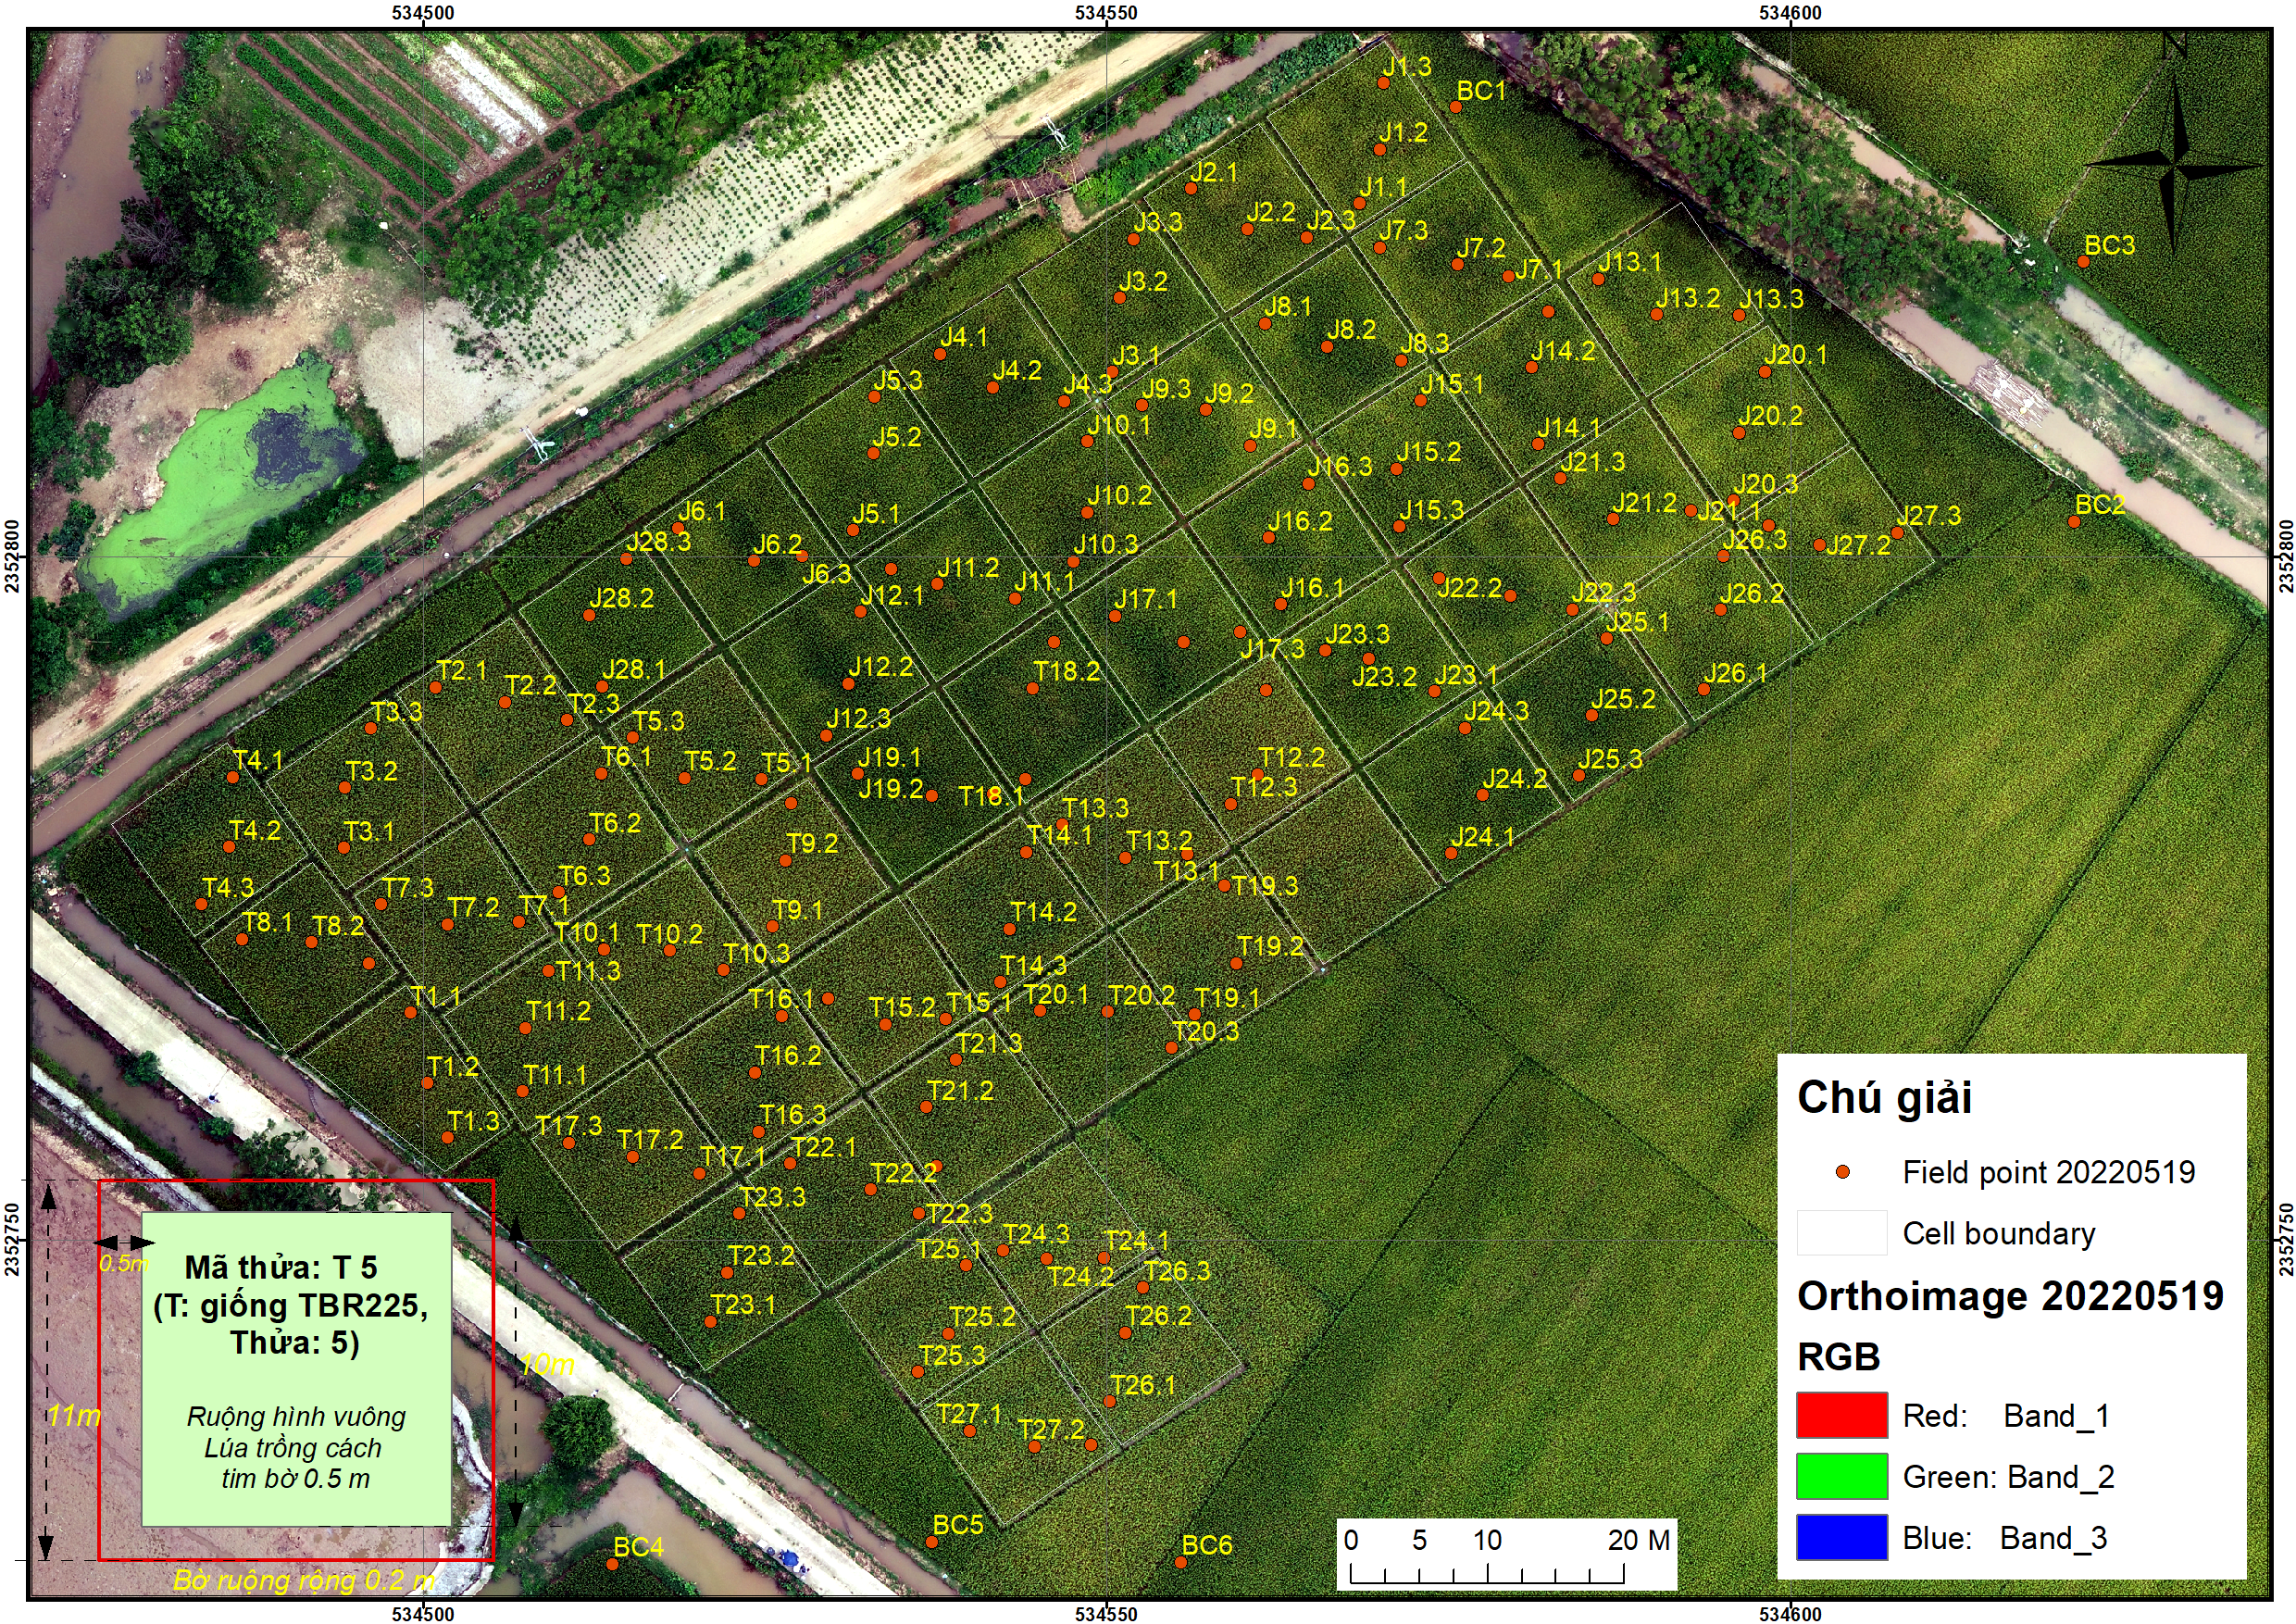
\includegraphics[width=1\textwidth]{image/Ground_mesurement_20220519.png}}
\caption{The sample field with 54 rice parcels} \label{fig:rice-field}
\end{figure}
    
    

\paragraph{Structure of .sed files} 
Number of .sed files: 260 files.
\begin{itemize}
    \item Content in a .sed file:
    \item Version: 2.3 [1.2.6250C]
    \item File Name
    \item Instrument: PSR-2500-SN1726293 [2]
    \item Detectors: 512,0,256
    \item Measurement: REFLECTANCE
    \item Date
    \item Time
    \item Temperature (c) 
    \item Battery Voltage
    \item Averages: 10,10
    \item Integration: 10,30,20,30
    \item Dark Mode: AUTO, AUTO
    \item Foreotopic: LENS {RADIANCE}, LENS4 {RADIANCE}
    \item Radiometric Calibration: RADIANCE
    \item Units: W/m2 /sr/nm
    \item Wavelength Range: 350,2500
    \item Latitude
    \item Longtitude
    \item Altitude
    \item GPS Time
    \item Satellites
    \item Calibrated Reference Correction File: none
    \item Channels: 2151
    \item Columns [4]

\end{itemize}

Each file also contain 2151 data, corresponding to wavelength channel captured from 350-2500 
\begin{itemize}
    \item Wavelength (Wvl)
    \item Reference Radian (Rad. (Ref.))
    \item Target Radian (Rad. (Target.))
    \item Reflect (Reflect.)
\end{itemize}

\paragraph{Structure of csv files}
There are 61 replicates, with 171 data row
\begin{itemize}
    \item Latitude
    \item Longitude
    \item Replicate, Sub-replicate
    \item Concentration of P, K (mg/kg)
    \item Chlorophyll-a
\end{itemize}

\begin{table}[H]
    \centering
    \begin{tabular}{c c c c c c} 
        \hline
        \textbf{Nutrients } & \textbf{Sample} & \textbf{Mean} & \textbf{Min} & \textbf{Max} & \textbf{St. Deviation}  \\
        \hline
        Chlorophyll  & 171 & 41.84 & 33.0 & 48.6 & 3.10  \\
        P concentration & 171 & 4317.11 & 1124.0 & 7740.0 & 805.68  \\
        K concentration & 171 & 35975.34  & 12620.0 & 59730.0 & 10578.94  \\
        \hline
    \end{tabular}
    \caption{Table of Nutrients’ statistics description} \label{table:mem-page-to-mem-size}
\end{table}
